\documentclass{article}
\usepackage{mainPoly}

\title{Fonction Exponentielle}
\date{}
\author{Premières Spécialité Mathématiques}

\begin{document}
\maketitle
\section{Définition de la fonction exponentielle}
\begin{tcolorbox}
\begin{definition}
La fonction exponentielle, notée $\exp$, est l'unique fonction définie sur $\R$ et à valeurs dans $\R$, dérivable sur $\R$, solution de l'équation différentielle
\begin{equation*}
f' = f
\end{equation*}
avec condition initiale $f(0) = 1$.
\end{definition}
\begin{remark}
\hfill
\begin{itemize}
\item \textbf{\og solution \fg} : La fonction $\exp$ est définie et dérivable sur $\R$, et, pour tout $x \in \R$, 
\begin{equation*}
\begin{cases}
\exp'(x) = \exp(x)\\
\exp(0) = 1
\end{cases}
\end{equation*}.
\item \textbf{\og unique \fg} : si une fonction $f \colon \R \to \R$ dérivable sur $\R$ vérifie que pour tout $x \in \R$, 
\begin{equation*}
\begin{cases}
f'(x) = f(x)\\
f(0) = 1\\ 
\end{cases}
\end{equation*}
alors $f = \exp$.
\end{itemize}
\end{remark}
\end{tcolorbox}
\begin{example}
\begin{enumquestions}
\item Soit $\function{g}{\R}{\R}{x}{x^2 - 3x + \exp(x)}$. Justifier que $g$ est dérivable sur $\R$, puis calculer sa dérivée.

\vspace*{0.5cm}
\emptybox{3cm}
\item Soit $\function{h}{\R}{\R}{x}{\exp(-5x+2)}$. Justifier que $h$ est dérivable sur $\R$, puis calculer sa dérivée.

\vspace*{0.5cm}
\emptybox{3cm}
\end{enumquestions}
\end{example}
\newpage

\section{Propriétés algébriques de l'exponentielle}
\begin{tcolorbox}
\begin{theorem}
Soit $x,y$ deux réels. Alors
\begin{equation*}
\exp(x + y) = \exp(x) \times \exp(y)
\end{equation*}
\end{theorem}
\end{tcolorbox}
\begin{remark}
\textbf{La fonction exponentielle transforme les sommes en produit.}
\end{remark}
\begin{proof}
Soit $y$ un nombre réel quelconque fixé. On pose $\function{g}{\R}{\R}{x}{\dfrac{\exp(x + y)}{\exp(x)}}$ (on admet que $\exp(x) > 0$ pour tout $x \in \R$).
\begin{enumquestions}
\item Justifier que $g$ est dérivable sur $\R$ et montrer que sa dérivée est nulle.
\item À l'aide de $g(0)$, en déduire la valeur de $g(x)$ pour tout $x \in \R$.
\item En conclure que $\exp(x + y) = \exp(x)\exp(y)$
\end{enumquestions}

\vspace*{0.5cm}
\emptybox{7cm}
\end{proof}
\begin{corollary}
Soit $x,y$ deux réels. Alors,
\begin{equation*}
\begin{cases}
\exp(x) \times \exp(-x) = 1\\
\exp(- x) = \dfrac{1}{\exp(x)}\\
\exp(x - y) = \dfrac{\exp(x)}{\exp(y)}
\end{cases}
\end{equation*}
\end{corollary}
\begin{proof}
On prouve $\exp(x - y) = \dfrac{\exp(x)}{\exp(y)}$ en admettant les deux identités précédentes.

\vspace*{0.5cm}
\emptybox{5cm}
\end{proof}
\newpage
\begin{tcolorbox}
\begin{definition}
Soit $a$ un réel. Alors la suite $(\exp(n \times a))_{n \in \N}$ est une \textbf{suite géométrique} de premier terme $1$ et de raison $\exp(a)$. On en déduit que pour tout $n \in \N$,
\begin{equation*}
\exp(na) = \exp(a)^n
\end{equation*}
\end{definition}
\end{tcolorbox}
\begin{proof}
On pose pour tout $n \in \N$, $u_n = \exp(na)$. Étudier $u_{n+1}$ en fonction de $u_n$, puis déduire que $(u_n)_{n \in \N}$ est géométrique.

\vspace*{0.5cm}
\emptybox{3cm}
\end{proof}
En particulier, on va s'intéresser à $a = 1$.
\begin{definition}
Le nombre $e = \exp(1)$ est appelé \textbf{constante de Néper}, et vaut approximativement \num{2,718}\dots

Par extension de la fonction puissance aux réels, la fonction exponentielle est notée, pour tout $x \in \R$,
\begin{equation*}
\exp(x) = e^x
\end{equation*}
\end{definition}
\begin{remark}
La raison pour laquelle la notation $e^x$ a été adoptée est pour correspondre avec les propriétés algébriques associées aux puissances :
\begin{equation*}
\begin{cases}
e^{x + y} = e^x e^y\\
e^{-x} = \dfrac{1}{e^x}\\
e^{x - y} = \dfrac{e^x}{e^y}\\
e^{nx} = (e^x)^n & \text{ pour tout } n \in \N 
\end{cases}
\end{equation*}
\end{remark}
\newpage
\section{Étude de la fonction exponentielle}
On représente sur ce repère la courbe représentative de la fonction exponentielle.
\begin{center}
\begin{tikzpicture}
\repereclassique{-5.25}{-5.25}{5.25}{5.25}{1};
\clip (-5.25,-5.25) rectangle (5.25,5.25);
\draw plot[samples=200,domain=-6:3] (\x,{exp(\x)});
\end{tikzpicture}
\end{center}
\begin{tcolorbox}
\begin{proposition}
La fonction exponentielle est strictement positive sur $\R$ : pour tout $x \in \R$,
\begin{equation*}
\exp(x) > 0
\end{equation*}
\end{proposition}
\end{tcolorbox}
\begin{tcolorbox}
\begin{proposition}
Le fonction exponentielle est strictement croissante sur $\R$ :
\begin{center}
\begin{tikzpicture}
\tkzTabInit{$x$/1, Variation de $\exp$/2}{$-\infty$,$0$,$+\infty$};
\tkzTabVar{-/,R/, +/};
\tkzTabIma{1}{3}{2}{$1$};
\end{tikzpicture}
\end{center}
\end{proposition}
\end{tcolorbox}
\end{document}